\documentclass{beamer}
\usepackage{amsmath}
\usepackage{amsopn}

\mode<presentation>{
\definecolor{cured}{rgb}{.8,0,.2}
\usecolortheme[named=cured]{structure}
%\usefonttheme{structurebold}
\usetheme{split}
}


\renewcommand{\emph}[1]{\textcolor{red}{\it #1}}


\newcommand{\GG}{\mathrm{GG}}
\newcommand{\YG}{\mathrm{YG}}
\newcommand{\RDG}{\mathrm{UDG}}

 
\usepackage{amsthm}

\newcommand{\centeripe}[1]{\begin{center}\Ipe{#1}\end{center}}
\newcommand{\comment}[1]{}

\newcommand{\centerpsfig}[1]{\centerline{\psfig{#1}}}

\newcommand{\seclabel}[1]{\label{sec:#1}}
\newcommand{\Secref}[1]{Section~\ref{sec:#1}}
\newcommand{\secref}[1]{\mbox{Section~\ref{sec:#1}}}

\newcommand{\alglabel}[1]{\label{alg:#1}}
\newcommand{\Algref}[1]{Algorithm~\ref{alg:#1}}
\newcommand{\algref}[1]{\mbox{Algorithm~\ref{alg:#1}}}

\newcommand{\applabel}[1]{\label{app:#1}}
\newcommand{\Appref}[1]{Appendix~\ref{app:#1}}
\newcommand{\appref}[1]{\mbox{Appendix~\ref{app:#1}}}

\newcommand{\tablabel}[1]{\label{tab:#1}}
\newcommand{\Tabref}[1]{Table~\ref{tab:#1}}
\newcommand{\tabref}[1]{Table~\ref{tab:#1}}

\newcommand{\figlabel}[1]{\label{fig:#1}}
\newcommand{\Figref}[1]{Figure~\ref{fig:#1}}
\newcommand{\figref}[1]{\mbox{Figure~\ref{fig:#1}}}

\newcommand{\eqlabel}[1]{\label{eq:#1}}
%\newcommand{\eqref}[1]{(\ref{eq:#1})}
\newcommand{\Eqref}[1]{Equation~(\ref{eq:#1})}

\newtheorem{thm}{Theorem}{\bfseries}{\itshape}
\newcommand{\thmlabel}[1]{\label{thm:#1}}
\newcommand{\thmref}[1]{Theorem~\ref{thm:#1}}

\newtheorem{lem}{Lemma}{\bfseries}{\itshape}
\newcommand{\lemlabel}[1]{\label{lem:#1}}
\newcommand{\lemref}[1]{Lemma~\ref{lem:#1}}

\newtheorem{cor}{Corollary}{\bfseries}{\itshape}
\newcommand{\corlabel}[1]{\label{cor:#1}}
\newcommand{\corref}[1]{Corollary~\ref{cor:#1}}

\newtheorem{obs}{Observation}{\bfseries}{\itshape}
\newcommand{\obslabel}[1]{\label{obs:#1}}
\newcommand{\obsref}[1]{Observation~\ref{obs:#1}}

\newtheorem{cond}{Condition}{\bfseries}{\itshape}

\newtheorem{clm}{Claim}{\bfseries}{\itshape}
\newcommand{\clmlabel}[1]{\label{clm:#1}}
\newcommand{\clmref}[1]{Claim~\ref{clm:#1}}


\newtheorem{dfn}{Definition}{\bfseries}{\rm}

\newtheorem{assumption}{Assumption}{\bfseries}{\rm}
\newenvironment{ass}{\begin{assumption}\rm}{\end{assumption}}
\newcommand{\asslabel}[1]{\label{ass:#1}}
\newcommand{\assref}[1]{Assumption~\ref{ass:#1}}

\newcommand{\proclabel}[1]{\label{alg:#1}}
\newcommand{\procref}[1]{Procedure~\ref{alg:#1}}

\newtheorem{rem}{Remark}
\newtheorem{op}{Open Problem}

\newcommand{\etal}{\emph{et al}}

%\newcommand{\keywords}[1]{\noindent\textbf{Keywords:} #1}
\newcommand{\voronoi}{Vorono\u\i}
\newcommand{\ceil}[1]{\left\lceil #1 \right\rceil}
\newcommand{\floor}[1]{\left\lfloor #1 \right\rfloor}
\newcommand{\R}{\mathbb{R}}
\newcommand{\N}{\mathbb{N}}
\newcommand{\Z}{\mathbb{Z}}
\newcommand{\Sp}{\mathbb{S}}
\newcommand{\E}{\mathrm{E}}

\usepackage{marvosym}

\newcommand{\notice}[1]
{
   {\Lightning}
   \marginpar{
      \begin{flushleft}\raggedright
        \hspace{-1.5mm}\Lightning{\small #1}
      \end{flushleft}
   }
}



\renewcommand{\etal}{\textit{et al}}

\newcommand{\pin}{p_{\mathsf{in}}}
\newcommand{\pout}{p_{\mathsf{out}}}
\DeclareMathOperator{\cost}{cost}
\DeclareMathOperator{\depth}{depth}

\title{On the Expected Maximum Degree \\ 
	of Yao Graphs}
\author{Luc Devroye 
	\and Joachim Gudmundsson
	\and Pat Morin}
\date{November 2, 2009 \\ Dagstuhl Seminar}

\begin{document}

\frame{\titlepage}

%\section[Outline]{}
%\frame{\tableofcontents}


\frame
{
  \frametitle{Yao Graphs (Yao 1982)}
  \begin{itemize}
    \item Defined on a set of points in $\R^2$
    \item For each point $u$, partition space around $u$ into $p$ cones,
           each of angle $2\pi/p$ and connect $u$ to nearest point in each cone
    \begin{center}
      \includegraphics{yao}
    \end{center}
    \item Yao graph has at most $pn$ edges and is a $t$-spanner
    \item Yao graph is also a $t'$ power spanner
  \end{itemize}
}

\frame
{
  \frametitle{Yao Graphs and Wireless Networks}
  \begin{itemize}
    \item $\YG\cap\RDG$ has at most $pn$ edges
    \item $\YG\cap\RDG$ is a $t'$ power spanner of the $\RDG$
    \item $\YG\cap\RDG$ can be computed locally
    \item This forms the basis of power-efficient routing protocols
    \begin{itemize}
          \item Li \etal\ 2001
          \item Bahl \etal\ 2001
    \end{itemize}
  \end{itemize}
}

\frame
{
  \frametitle{Random Yao Graphs}
  \begin{itemize}
    \item Place $n$ point u.i.d. in a unit square
    \item What can you say about $\YG$? \\
          \textbf{Theorem 1:}
           For a set of $n$ points uniformly and independently distributed
		in \emph{a} unit square,
           \[\lim_{n\rightarrow\infty}
              \Pr\left\{\mbox{Maximum degree} \in \Theta\left(\frac{\log
n}{\log\log n}\right)\right\} = 1 \]
  \end{itemize}
}


\frame
{
  \frametitle{Random Yao Graphs}
  \begin{itemize}
    \item We will prove Theorem 1 for Yao graphs with $p=4$
    \begin{center}
      \includegraphics{yao-2}
    \end{center}
    \item We focus on upper-right neighbours
    \item For the upper bound we will use points u.i.d. in the unit 
          square rotated by $45^\circ$
  \end{itemize}
}


\frame
{
  \frametitle{A Special Value}
  \begin{itemize}
    \item Let $k=c\log n / \log\log n$
      \begin{itemize}
        \item Then
         \[ k^k = n^{c(1 + \frac{\log c-\log\log\log n}{\log\log n})} \]
        \item In particular, for any $\epsilon > 0$,
         \[ k^k = O(n^c) \]
         and 
         \[ k^k = \Omega(n^{c-\epsilon}) \]
      \end{itemize}
  \end{itemize}
}

\frame
{
  \frametitle{The Lower Bound: $(k,r)$-Staircases}

  \begin{center}
    \includegraphics{staircase}
  \end{center}
  \begin{itemize}
    \item A $(k,r)$ staircase (at $x$) includes one point in each step
          and no points anywhere else
    \item In a Yao graph (with $p=4$), $x$ will have degree at least $k$
  \end{itemize}
}


\frame
{
  \frametitle{$(k,r)$-Staircases --- Conditional}

  \begin{center}
      \includegraphics[height=1.2in]{condition} 
  \end{center}
  \begin{itemize}
    \item Let $X_1,\ldots,X_n$ be i.u.d. in $[0,1]^2$
    \item $r=\sqrt{2/n}$, and $k=c\log n/\log\log n$, then
    \begin{eqnarray*}
     \Pr\{\mbox{$(k,r)$-staircase at $X_1$}| X\in[r,1-r]^2\} 
         & \ge & 1/(k^2)^k \\
         & = & \Omega(1/n^{2c}) 
    \end{eqnarray*}
  \end{itemize}
}

\frame
{
  \frametitle{$(k,r)$-Staircases --- Unconditioning}

  \begin{itemize}
    \item The condition $X_1\in [r,1-r]^2$ is easily removed:
    \[
      \Pr\{\mbox{$(k,r)$-staircase at $X_1$}\} 
        \ge (1-2r)^2 \Omega(1/n^{2c}) 
        = \Omega(1/n^{2c})
    \]
    so 
    \[ \E[\mbox{\#$(k,r)$-staircases}] = n\Pr\{\mbox{$(k,r)$-staircase at $X_1$}\}
      = \Omega(n^{1-2c}) \]
  \end{itemize}
}

\frame
{
  \frametitle{Lower Bound --- Summary}

  \begin{itemize}
    \item Each $(k,r)$-staircase creates vertex of degree at least $k$
    \item $\E[\mbox{\# vertices of degree $\ge k$}]=\Omega(n^{1-2c})$
    \item $\E[\mbox{\# vertices of degree $\ge k$}]\rightarrow\infty$ 
          for $c < 1/2$
    \item This almost proves:\\
       \textbf{Theorem 1a:}
           For a set of $n$ points uniformly and independently distributed
		in a unit square, 
           \[\lim_{n\rightarrow\infty}
              \Pr\left\{\mbox{Max degree} > \frac{c\log
n}{\log\log n}\right\} = 1 \]
           for any $c < 1/4$.
    \item Finish the proof using the second moment method
  \end{itemize}
}

\frame
{
  \frametitle{Upper Bound (Sketch)}

  \begin{center}
    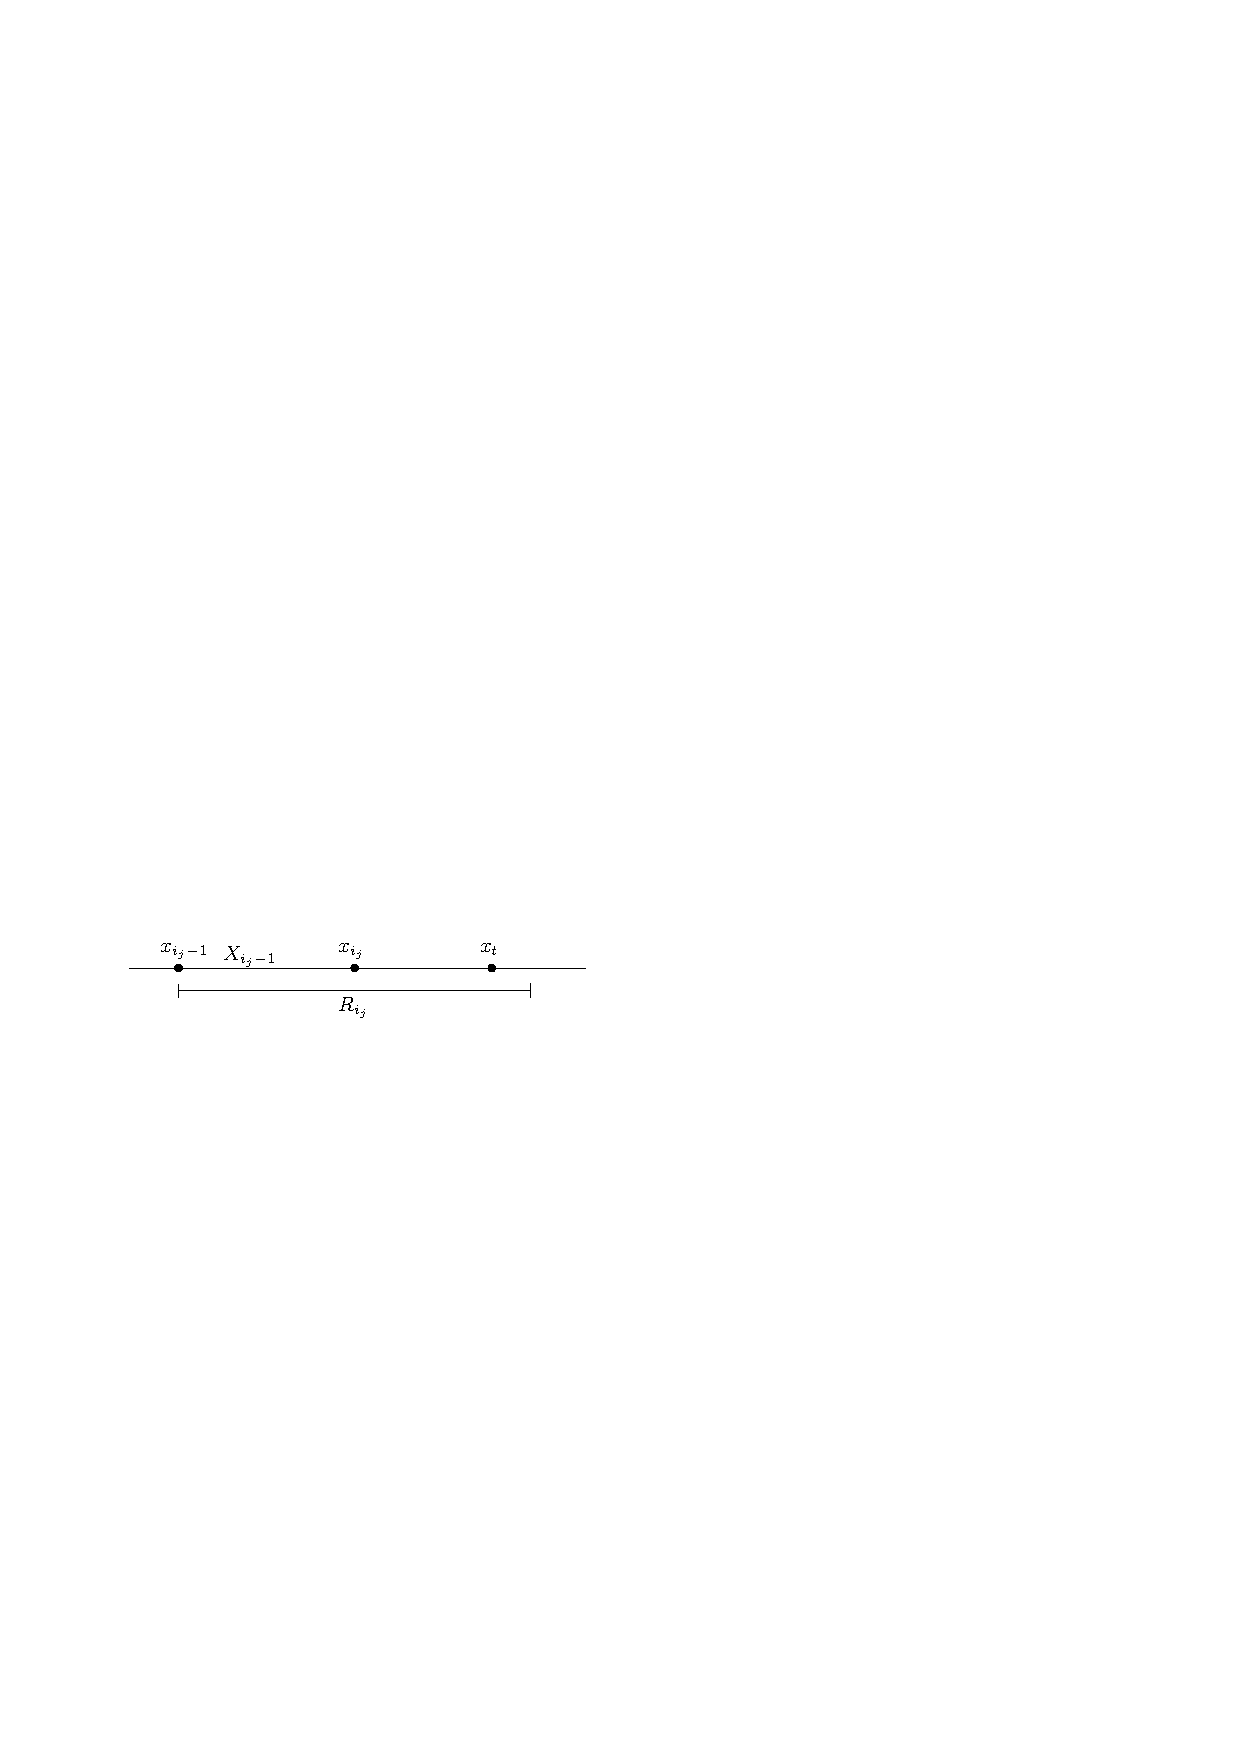
\includegraphics[height=1.2in]{upper-bound}
  \end{center}
  \begin{itemize}
    \item Consider neighbours of $X_1$ that are \emph{close to} to $X_1$
    \item Show that $\Pr\{N_\mathrm{close} > c\log n/\log\log n\} \le 1-a$
    \item Show that $\Pr\{N_\mathrm{far} > 0\} \le 1-b$
    \item With probability at least $1-4n(a+b)$,
no vertex has degree greater than $4c\log n/\log\log n$
  \end{itemize}
}

\frame
{
  \frametitle{Chernoff's Bounds}

    \textbf{Lemma (Chernoff 1952):}
    Let $Y_1,\ldots,Y_m$ be a sequence of independent $\{0,1\}$-valued
    random variables, let $Y=\sum_{i=1}^m Y_i$, and let $\mu=\E[Y]$.
    Then, for any, $\delta > 0$,
    \[
       \Pr\{Y > (1+\delta)\mu\} 
         \le \left(\frac{e^{\delta}}{(1+\delta)^{(1+\delta)}}\right)^{\mu}
    \]
}

\frame
{
  \frametitle{Close Points}


   \begin{itemize}
     \item
       \textbf{Lemma:} The number of points ``close to'' $X_1$ is at most
$2d\log n$, with probability at least $1-1/n^{\Omega(d)}$

     \item \textbf{Proof:} Use Chernoff's Bounds.
     \item How many of these points are neighbours of $X_1$?
     \end{itemize}
}

\frame
{
  \frametitle{Neighbours and Minima}

   \begin{itemize}
     \item The neighbours of $X_1$ are all \emph{minima}
      \begin{center}
        \includegraphics[height=1.2in]{minima-x}
      \end{center}
     \item Minima have been studied extensively
   \end{itemize}

}

\frame
{
  \frametitle{Review of Results on Minima}

   \begin{center} \includegraphics[height=1in]{minima} \end{center}
   \begin{itemize}
     \item Place $m$ points $Z_1,\ldots,Z_m$ uniformly in a unit square$^{*}$
     \item $\E[\mbox{\#minima}] =\sum_{i=1}^m 1/i \le \ln n + 1$
     \item $\Pr\{\mbox{\#minima} > (1+\delta)(\ln m +1)\} \le 
         \left(\frac{e^{\delta}}{(1+\delta)^{(1+\delta)}}\right)^{\ln m}$
   \end{itemize}
}

\frame
{
  \frametitle{Minima and Neighbours}

   \begin{itemize}
     \item For us, $m=2d\log n$, so $\E[\mbox{\#minima}] \le \ln(2d\log n) +1$
     \item We want to bound $\Pr\{\mbox{\#minima} > c\log n/\log\log n\}$
     \item $\Pr\{\mbox{\#minima} > (1+\delta)(\ln m +1)\} \le 
         \left(\frac{e^{\delta}}{(1+\delta)^{(1+\delta)}}\right)^{\ln m}$
     \item We get, for any $\epsilon > 0$,
       \[\Pr\{\mbox{\#minima} > c\log n/\log\log n\}
         \le O(1/n^{c/4-\epsilon}) \]
   \end{itemize}
}

\frame
{
  \frametitle{The Lie}

   \begin{itemize}
     \item The points ``close to'' $X$ may not be u.i.d. in a square (or
rectangle even)
      \begin{center}
        \includegraphics{lie} 
      \end{center}
     \item Can handle this by decomposing into $O(1)$ rectangles and using
           a symmetry argument
   \end{itemize}
}




\frame
{
  \frametitle{Review so Far}

  \begin{center}
    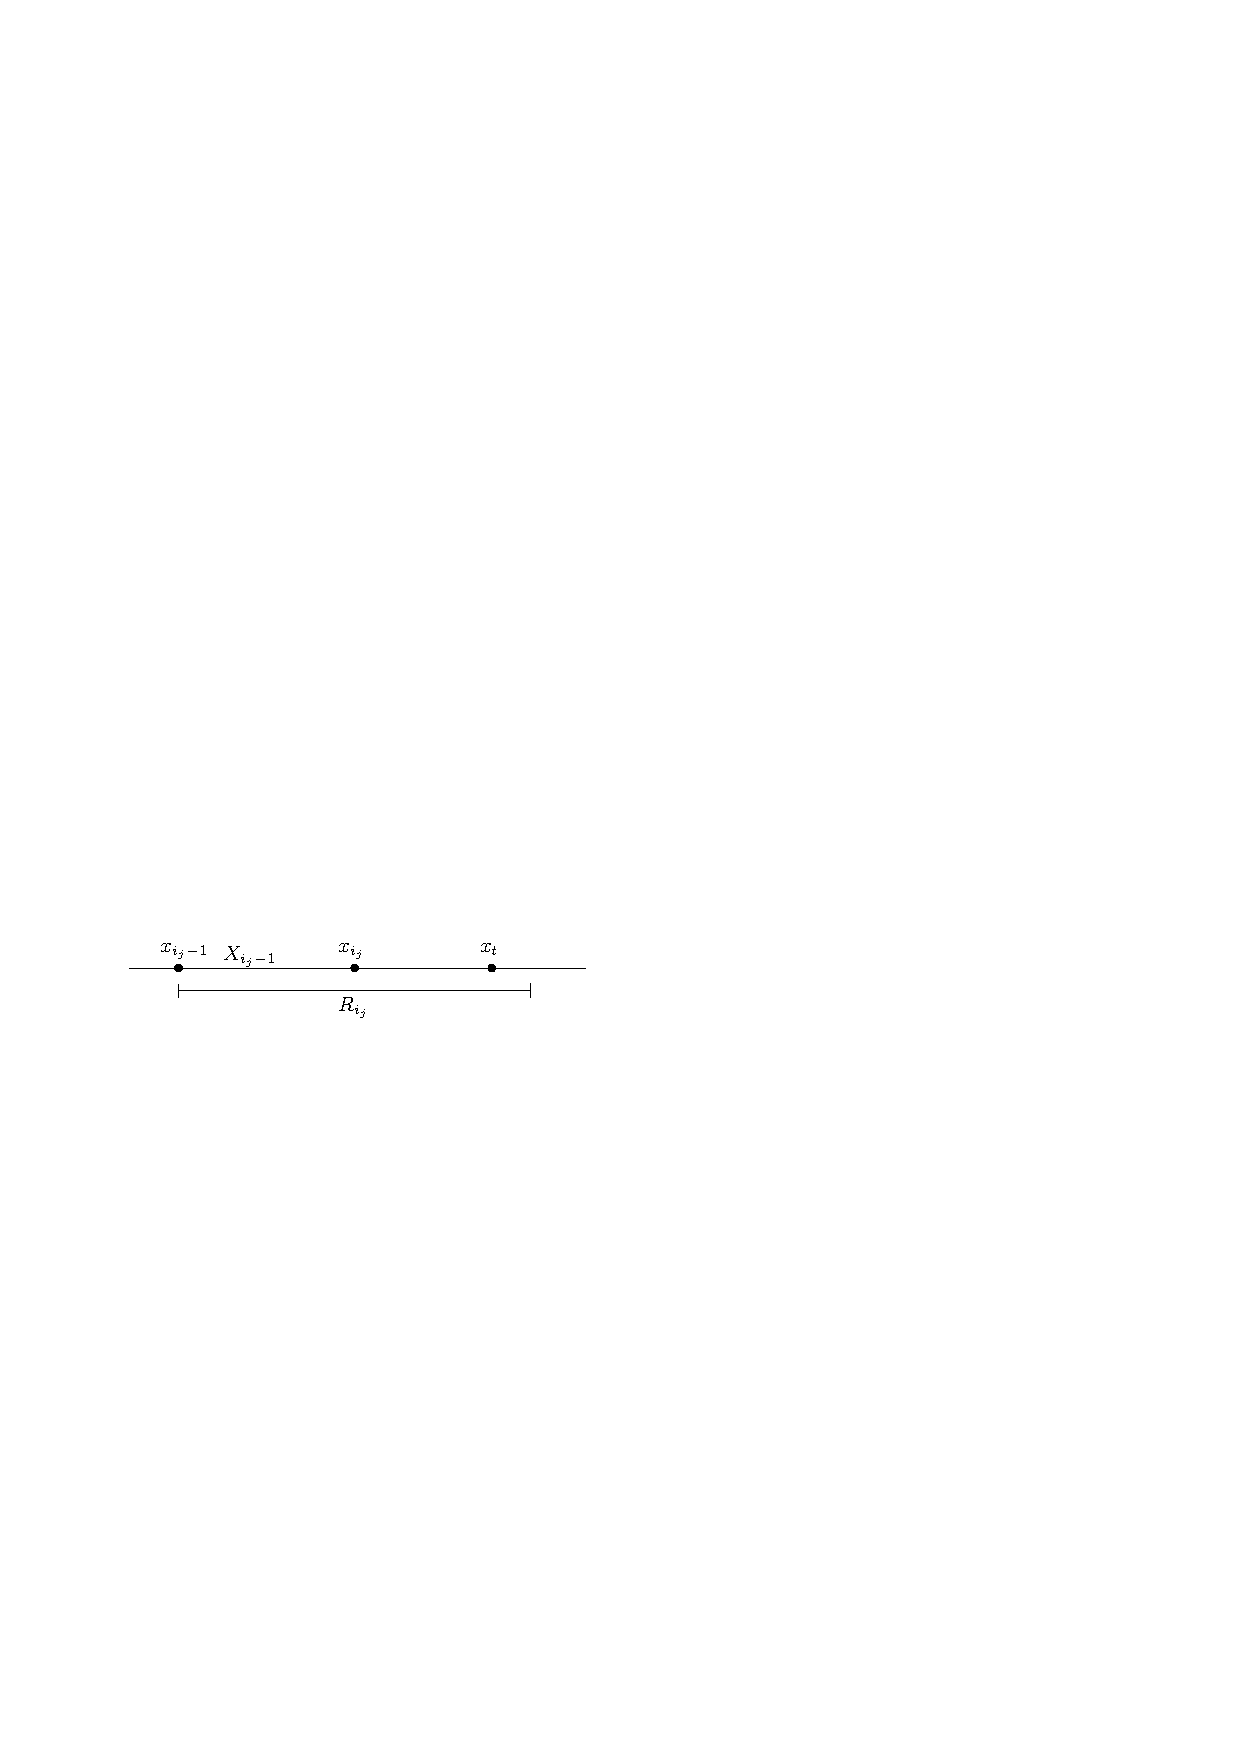
\includegraphics[height=1.2in]{upper-bound}
  \end{center}
   \begin{itemize}
     \item So far we know
       \[
         \begin{aligned}
          &\Pr\{\mbox{$X_1$ has more than $c\log n/\log\log n$ close neighbours}\} \\
          & \le 1/n^{\Omega(d)} + O(1/n^{c/4-\epsilon}) 
         \end{aligned}
       \]
     \item What about neighbours that are ``far from'' $X_1$?
   \end{itemize}
}


\frame
{
  \frametitle{Far Neighbours}

  \begin{center}
    \begin{tabular}{cc}
      \includegraphics[height=1.2in]{far} &
	\includegraphics[height=1.2in]{empty2}
    \end{tabular}
  \end{center}
   \begin{itemize}
     \item A far neighbour defines an empty region of area at least
           $(\pi d\log n)/4n$
     \item At least $d\log n/4n$ of this region is in the support set
       \[
         \begin{aligned}
          &\Pr\{\mbox{$X_2$ is a far neigbour of $X_1$}\} \\
          & \le (1-(d\log n)/4n)^{n-2}
          & \le (1/e)^{\Omega(d\log n)}
          & \le 1/n^{\Omega(d)}
         \end{aligned}
       \]
      \item 
       $\Pr\{\mbox{$X_1$ has any far neighbour}\} 
           \le n/n^{\Omega(d)} 
           = 1/n^{\Omega(d)}$
   \end{itemize}
}

\frame
{
  \frametitle{Finishing Up}

   \begin{itemize}
     \item So far we know
       \[
         \begin{aligned}
          &\Pr\{\mbox{$X_1$ has more than $c\log n/\log\log n$ neighbours}\} \\
          & \le 1/n^{\Omega(d)} + O(1/n^{c/4+\epsilon}) + 1/n^{\Omega(d)}  
         \end{aligned}
       \]
     \item So,
       \[
         \begin{aligned}
          &\Pr\{\mbox{any vertex has more than $c\log n/\log\log n$ neighbours}\} \\
          & \le n(1/n^{\Omega(d)} + O(1/n^{c/4+\epsilon}) + 1/n^{\Omega(d)}) \\
          & = 1/n^{\Omega(d)} + O(1/n^{c/4-1+\epsilon}) \rightarrow 0
         \end{aligned}
       \]
      for large enough $d$ and $c>4$.
   \end{itemize}
}

\frame
{
  \frametitle{Finishing Up}


       \textbf{Theorem 1b:}
           For a set of $n$ points uniformly and independently distributed
		in a $45^\circ$-rotated unit square, 
           \[\lim_{n\rightarrow\infty}
              \Pr\left\{\mbox{Max degree} < \frac{c\log
n}{\log\log n}\right\} = 1 \]
           for any $c > 4$.

}

\frame
{
  \frametitle{Summary}

    \textbf{Theorem 1:}
     For a set of $n$ points uniformly and independently distributed
		in a ($45^\circ$-rotated) unit square, 
     \[\lim_{n\rightarrow\infty}
         \Pr\left\{\mbox{Max degree} 
           \in \Theta\left(\frac{\log n}{\log\log n}\right)\right\} = 1 
     \]

    \begin{itemize}
      \item Theorem 1 holds for Yao graphs with any constant value of $p$
         and Gabriel graphs in any constant dimension $d$.
      \item Must avoid axes of square aligning with
	sides of the cones or 
      \item consider only points at distance
         $\Omega(\sqrt{(\log n)/n})$ from the boundary
    \end{itemize}


}


\frame{
   \frametitle{Open Problem}

   \noindent\textbf{Open Problem:} What is the expected maximum degree of a Yao graph
for $n$ points u.i.d. in $[0,1]^d$?

  \begin{itemize}
   \item Lower bound of $\Omega(\log n/\log\log n)$ still holds but upper
bound is missing
  \end{itemize}
}




\end{document}

